% SAFA --- IEEE Open Journal template (IEEE-open-journal-template.zip: ieeetj.cls,
% tj-template-s1.tex conventions). English version of sn-article.tex.
% Keep terminology consistent with the Korean version.
% ieeetj.cls is included in the repo (identical to the zip). Uppercase section
% titles, \IEEEPARstart, and front matter follow the template conventions.
\documentclass{ieeetj}

\usepackage{graphicx}
\usepackage{amsmath,amssymb,amsfonts}
\newcommand{\cmark}{\ensuremath{\checkmark}}   % table: public
\newcommand{\xmark}{\ensuremath{\times}}        % table: closed/none
\usepackage{amsthm}
\usepackage{mathrsfs}
\usepackage{booktabs}
\usepackage{multirow}
\usepackage{tabularx}         % Table 1: auto-width wrapping columns (keeps it inside \textwidth)
\newcolumntype{Y}{>{\raggedright\arraybackslash}X}
\usepackage{xcolor}
\usepackage{algorithm}
\usepackage{algpseudocode}
\usepackage{algcompatible}   % uppercase macros \STATE \IF \FOR etc. (Algorithm 1)
\providecommand{\RETURN}{\State \Return}  % some TeXLive algcompatible lacks \RETURN -> supply (ignored if defined)
\usepackage{cite}
\usepackage{placeins}         % \FloatBarrier — keep figures inside section/bibliography boundaries
\usepackage{subcaption}       % 2x2 concept diagram (subfigures)
\usepackage[hidelinks]{hyperref}
\usepackage{orcidlink}       % author ORCID icons (\orcidlink)
\AtBeginDocument{\definecolor{tmlcncolor}{cmyk}{0.93,0.59,0.15,0.02}\definecolor{NavyBlue}{RGB}{0,86,125}}
\def\OJlogo{\vspace{-4pt}}
\def\seclogo{\vspace{10pt}}
\def\authorrefmark#1{\ensuremath{^{\textbf{#1}}}}

\newtheorem{theorem}{Theorem}
\newtheorem{proposition}[theorem]{Proposition}
\newtheorem{definition}{Definition}
\newtheorem{remark}{Remark}

\begin{document}

\receiveddate{XX Month, XXXX}
\reviseddate{XX Month, XXXX}
\accepteddate{XX Month, XXXX}
\publisheddate{XX Month, XXXX}
\currentdate{XX Month, XXXX}
\doiinfo{XXXX.XXXX.0000000}

\markboth{SAFA: Resolving Head-of-Line Blocking in GPU Cluster Job Queues with Prediction-Free Reordering}{Cho \MakeLowercase{et al.}}

\title{SAFA: Resolving Head-of-Line Blocking in GPU Cluster Job Queues with Prediction-Free Reordering}

\author{Kyunam~Cho\authorrefmark{1}\authorrefmark{2}\,\orcidlink{0000-0002-8300-8192}, YoungHwan~Jin\authorrefmark{2}\,\orcidlink{0000-0001-9302-9897}, and Heonchang~Yu\authorrefmark{1}\,\orcidlink{0000-0003-2216-595X}}
\affil{Department of Computer Science and Engineering, Korea University, Seoul, Republic of Korea}
\affil{LG Uplus Corp., Seoul, Republic of Korea}
\corresp{Corresponding author: Heonchang Yu (e-mail: yuhc@korea.ac.kr).}
\authornote{K. Cho e-mail: mystous@korea.ac.kr. Y. Jin e-mail: yhjin@korea.ac.kr.}

\begin{abstract}
Most training jobs in production GPU clusters now ask for several GPUs at once, and often for an entire node. A gang-scheduled job of this kind cannot start until every GPU it asked for is free at the same time. As jobs of different sizes come and go, the free GPUs scatter across nodes. A cluster can then hold plenty of idle capacity and still have no single node with room for a large job. That job waits at the front of the queue, and because the queue is served in order, every job behind it waits too. This is Head-of-Line (HOL) blocking. It leaves GPUs idle that the waiting jobs could have used, and a large job can be passed over for so long that it never runs at all. Schedulers decide two things in turn. The Order stage picks which queued job to consider next. The Placement stage picks where that job runs. HOL blocking is therefore an ordering problem, since only the Order stage decides whether a blocked job holds up the rest. We present SAFA (Starvation-Aware Fair Aging), which changes only the Order stage. SAFA looks at four numbers it can read directly when it makes a decision, namely where a job sits in the queue, how many GPUs it wants, how long it has waited compared with its neighbors, and how many GPUs each server has free. It predicts nothing, profiles nothing, and solves nothing. What it does need is a balance, since reordering too aggressively would trade one kind of unfairness for another, so a coefficient governs how far a waiting job may be promoted. SAFA derives this coefficient from the queue's own statistics, so it needs no retuning when the workload changes. We replay the 111k-job Philly trace under heavy overload. All six Order policies fall to an order-fairness score of 0 out of 100. Four of them were given information SAFA never receives, either the runtimes the trace recorded after the fact or a reconstructed utilization profile, and they collapsed anyway. SAFA scores 92.7 to 93.5 on the same measure. It also shortens the median queue wait by 7 to 13\% against FIFO and lifts average GPU utilization from 92\% to 95 or 96\%, so the fairness comes at no cost in throughput. The same pattern holds on Helios and Alibaba, two traces from unrelated clusters. On a live NVIDIA B200$\times$8 Kubernetes cluster, SAFA again keeps large jobs from being passed over. SAFA never touches placement, so it can run ahead of any Placement policy. We tried seven Placement policies, and under each one SAFA raised the allocation rate over FIFO by 3.7 to 5.8 percentage points. The gain was largest under KAI spread, the policy that scatters free GPUs most widely and therefore wastes the most to fragmentation.
\end{abstract}

\begin{IEEEkeywords}
Datacenter GPU, GPU gang scheduling, head-of-line blocking, order fairness, pre-placement reordering layer, prediction-free scheduling, queue reordering, tuning-free scheduling.
\end{IEEEkeywords}

\maketitle


\section{INTRODUCTION}\label{sec1}
\IEEEPARstart{J}{ob} scheduling in GPU clusters has long been studied as a central problem because it directly affects both operational and research costs. Large organizations build ``hyper-clusters'' that interconnect hundreds to thousands of GPUs through high-bandwidth links. As a continuous stream of jobs with disparate GPU demands and job completion times (JCTs) arrives, cluster resources become fragmented\cite{athlur2022varuna}. Fragmentation is even more severe in shared environments that use fractional GPUs, where hundreds of GPUs may remain idle across the cluster yet still be unavailable to new jobs\cite{weng2023beware}. Scheduling alone cannot fully resolve this problem. Even when every job's runtime is known in advance, assigning queued jobs to machines is NP-hard\cite{ullman1975np}, and GPU cluster scheduling inherits this hardness from the classical parallel-machine problems it generalizes\cite{b1}. A datacenter scheduler does not even have that much, since runtimes are unknown at submission, which makes the problem harder still and leaves approximation as the only practical recourse\cite{b2}.

Schedulers for deep-learning jobs have nonetheless improved substantially. Ye et al.\cite{b3} survey the field and identify two representatives of the current state of the art, Sia\cite{b4}, which leads on utilization, fairness, and completion time simultaneously, and Lucid\cite{b5}, which raises throughput through multi-state profiling. Most contemporary GPU schedulers are variants of one or the other. They all rest on quantities that cannot be observed when the scheduling decision is made, and must instead be predicted, profiled, or solved for. Optimus\cite{peng2018optimus} and other elastic schedulers need online performance models. These models carry up to 20\% error in convergence estimation and force a checkpoint whenever resources are reconfigured. Themis\cite{mahajan2020themis} needs a centralized auction solver and bids supplied by the applications themselves. The learning-to-rank scheduler of Fu et al.\cite{fu2024efficient} needs a predicted output-length ranking. The two leading systems are no exception, since both Sia and Lucid need per-job throughput profiles. Acquiring any of this costs profiling time, prediction error, or dedicated infrastructure, and none of it survives a change in workload without refitting.

To address these drawbacks, this work proposes Starvation-Aware Fair Aging (SAFA). SAFA decides from quantities that are already on hand at the scheduling instant, namely each pending job's position in the queue, its resource demand, its age relative to the other pending jobs, and the free-GPU count on each server. Nothing here is estimated or learned, so SAFA needs no runtime estimate, no throughput profile, and no solver. SAFA does not attack the scheduling problem as a whole. It targets one failure mode, the Head-of-Line (HOL) blocking\cite{karol1987hol} that resource fragmentation induces. HOL blocking was first characterized in packet switching, where a blocked head-of-queue packet stalls every packet behind it. A GPU server pool reproduces both halves of that pattern. Fragmentation leaves the head job without a server large enough to hold its gang, and a queue served in arrival order passes that failure on to every job waiting behind it. SAFA leaves the core scheduler unchanged while mitigating the queueing delay and arrival-order unfairness that HOL blocking induces. Its key contributions are as follows.

\begin{enumerate}
\item Prediction-free reordering that prevents indefinite exclusion: SAFA reorders the queue from queue position, accumulated age, resource demand, and current server occupancy alone, cutting HOL-induced queueing delay without discarding arrival order. Because the reordering weighs each job's accumulated age against its fitness for the currently vacant slots, a large job is never excluded outright. Jobs that fit the vacant slots move up, while the large job keeps accumulating age and rises in priority relative to the rest of the queue.
\item Placement composability: SAFA handles only the Order stage, which determines which job is served first, and leaves the Placement stage, which determines where the selected job is placed, unchanged. It can therefore sit unchanged ahead of diverse Placement policies and does not require replacement of the core scheduler. This composability holds across all seven Placement policies (most-allocated, compact, round-robin, MCTS, FGD, KAI binpack, and KAI spread), and the more strongly a placement policy scatters jobs and induces fragmentation, the more resources SAFA recovers from HOL blocking.
\item Tuning-free coefficient: A coefficient $\alpha$ governs how far a waiting job may be promoted, and thus the trade-off between resolving HOL blocking and preserving fairness. Because $\alpha$ is normalized using observed queue-age statistics and resource fitness and determined dynamically, SAFA eliminates the tuning knob and adapts to workload change without a new grid search.
\end{enumerate}

The remainder of this paper is organized as follows. Section~\ref{Related} reviews related work. Section~\ref{motivation} motivates the need for queue reordering. Section~\ref{algo:intro} presents the mathematical formulation of queue reordering and its tuning-free balancing mechanism. Section~\ref{sec:eval} evaluates SAFA using public traces (Philly, Helios, Alibaba) and real B200 Kubernetes measurements. Finally, Section~\ref{conclu} summarizes the findings and outlines future directions.

Throughout this paper, ``GPU'' denotes a datacenter GPU, and we use the shorter term for brevity.

\section{RELATED WORK}\label{Related}
To position SAFA relative to prior work, we distinguish existing studies along two dimensions. The first is the stage at which a scheduler intervenes. Although scheduling can be decomposed in several ways, the relevant stages fall broadly into an Order stage, which determines which job is served first, and a Placement stage, which determines where the selected job is placed. The second dimension is whether every quantity the decision depends on can be observed at the moment the decision is made. Queue position, resource demand, accumulated waiting, observed cumulative usage, and current node occupancy are all available on inspection. Anything else must be predicted, profiled, or solved for, and we divide such derived quantities into three categories, namely runtime estimation or rank prediction (SJF, EASY backfilling, learning-to-rank), per-job performance or throughput profiles (Optimus, Lucid, Sia, Pollux, Arena, Rubick), and round solvers or auction bids (Themis, FFT, RLTune).

Two forms of FIFO recur throughout this paper and must be kept apart. Blocking FIFO serves jobs strictly in arrival order, so a head job that cannot be placed halts the entire queue. Non-blocking FIFO scans past the blocked head and dispatches the first job that fits. The second form recovers the idle GPUs that the first wastes, but it no longer preserves arrival order, and a large job it repeatedly skips can be starved indefinitely.

\begin{table*}[htb!]
\centering
\caption{Taxonomy of schedulers}
\label{tab:related}
\scriptsize
\setlength{\tabcolsep}{4pt}
\begin{tabularx}{\textwidth}{@{}llYcY@{}}
\toprule
\textbf{System} & \textbf{Venue} & \textbf{Decision axis (information assumption)} & \textbf{Exp.} & \textbf{Rationale / representative baseline} \\
\midrule
\multicolumn{5}{@{}l}{\textit{Experimental baselines --- same layer, information budget never below SAFA's}}\\
FIFO (blocking) & --- & queue order (observed only) & $\checkmark$ & control (pure policy effect)\\
SJF & classic & queue order (oracle duration) & $\checkmark$ & mean-optimal reference\\
LAS (Tiresias)\cite{gu2019tiresias} & NSDI'19 & queue order (attained service) & $\checkmark$ & least-attained\\
Kueue\cite{kueue2024} & k8s & quota gate (observed only) & $\checkmark$ & production standard\\
EASY\cite{mualem2001backfilling} & HPC & reservation+backfill (oracle duration) & $\checkmark$ & perfect-estimate variant (not an upper bound)\\
Themis\cite{mahajan2020themis} & NSDI'20 & FTF ordering (oracle duration, $\pm20\%$; solver omitted) & $\checkmark$(adapted) & fairness axis; round auction not reproduced\\
Lucid\cite{b5} & ASPLOS'23 & profile packing & $\checkmark$(adapted) & synthetic utilization, duration-oracle injection --- a single scalar bounds the synthesis distortion\\
\textbf{SAFA} & --- & queue order + node occupancy (observed only) & $\checkmark$ & this work (prediction-free)\\
\midrule
\multicolumn{5}{@{}l}{\textit{Orthogonal Placement axis --- prediction-free like SAFA, composed rather than compared}}\\
FGD\cite{weng2023beware} & ATC'23 & Placement (fragmentation avoidance; observed only) & $\checkmark$ & complementary stage; SAFA$\oplus$FGD composition\\
KAI\cite{kai2025} & k8s & Placement (binpack/spread; observed only) & $\checkmark$ & production standard; SAFA$\oplus$KAI composition\\
\midrule
\multicolumn{5}{@{}l}{\textit{Related work --- decision variables absent from traces or layer mismatch}}\\
Learning-to-Rank\cite{fu2024efficient} & NeurIPS'24 & LLM request order (predicted rank, ms) & --- & layer mismatch; represented by SJF\\
NotebookOS\cite{notebookos2026} & ASPLOS'26 & interactive replication & --- & different workload (out of scope)\\
Sia\cite{b4} & SOSP'23 & elastic ILP (goodput profiles) & --- & profile decision variables absent from traces\\
Gavel\cite{narayanan2020gavel} & OSDI'20 & heterogeneity-aware round policy (throughput matrix) & --- & throughput-matrix decision variables absent\\
Optimus\cite{peng2018optimus} & EuroSys'18 & elastic worker/PS (performance model) & --- & performance-model decision variables absent\\
Pollux\cite{qiao2021pollux} & OSDI'21 & elastic goodput (profiles) & --- & goodput profiles absent\\
Arena\cite{arena2026} & EuroSys'26 & adaptive parallelization (profiles+estimates) & --- & execution-plan decision variables absent\\
Rubick\cite{rubick2025} & MLSys'25 & execution-plan reconfiguration & --- & execution-plan decision variables absent\\
RLTune\cite{rltune2025} & SoCC'25 & RL ordering+MILP (learned model) & --- & learning+solver; represented by Lucid/Themis\\
FFT\cite{fft2025} & ICS'25 & round cost-min (epoch estimates) & --- & solver+estimates; represented by Themis (FTF)\\
Tetris\cite{grandl2014multi} & SIGCOMM'14 & multi-dimensional resource alignment (order$+$placement) & --- & decision variables absent; couples Placement\\
Maui\cite{jackson2001maui} & JSSPP'01 & multi-factor priority (runtime, fairshare) & --- & requires estimates and usage history; residual aging reduces to FIFO\\
\bottomrule
\end{tabularx}
\end{table*}

\subsection{Techniques by Scheduling Stage}
We begin with the Order stage. Kueue\cite{kueue2024} is a Kubernetes-native queueing system that suspends and resumes jobs and provides quota-based fair sharing. Because it operates purely as a gating layer without replacing the core scheduler, it serves as this paper's most direct production-standard baseline. Its fairness mechanism, however, is limited to quota distribution and addresses neither HOL starvation nor fragmentation. Moreover, quota fairness becomes relevant only under multi-Virtual-Cluster (VC) contention, and within a single VC Kueue reduces to non-blocking FIFO. LAS in Tiresias\cite{gu2019tiresias} is a prediction-free discipline that favors jobs with the least accumulated resource usage and, when combined with multi-level feedback queues and preemption, reduces the mean JCT. Under non-preemptive GPU operation, however, pending jobs retain an accumulated resource usage of 0, so the ordering key carries no information and LAS likewise reduces to non-blocking FIFO. This behavior may differ from the original Tiresias setting, in which preemption is central.

Two methods lie on the Placement axis. FGD\cite{weng2023beware}, designed for shared clusters heavily fragmented by partial GPU occupancy (21 to 42\% in traces), estimates the probability that a randomly drawn job cannot be scheduled, places each job on the node whose placement raises that probability the least, and reduces unallocated GPUs by up to 49\%. Like SAFA, it decides from queue state and node occupancy alone and predicts nothing. It differs in the stage it occupies. FGD chooses where a job goes once the job has been selected, and therefore cannot help a head job for which no node is large enough. That case is what SAFA addresses, so the two are complementary rather than competing, and we evaluate FGD as a composition target. The production scheduler KAI\cite{kai2025} provides binpack and spread modes. Its default binpack mode assigns higher scores ($\text{score}\propto 1-(\text{free}-\min)/(\max-\min)$) to nodes with fewer unallocated GPUs, thereby consolidating jobs and preserving empty nodes for large gangs.

\subsection{Techniques Relying on Derived Quantities}
We group techniques that depend on quantities unavailable at decision time into three categories, namely (i) runtime estimation and rank prediction, (ii) per-job performance or throughput profiles, and (iii) round solvers and auction bids. These categories are ordered by increasing acquisition cost, counting estimation error, profiling overhead, and dedicated infrastructure.

(i) Runtime estimation and rank prediction: EASY backfilling\cite{mualem2001backfilling} is the standard HPC technique that reserves resources for the queue head while advancing later jobs only when doing so does not disturb the reservation. It depends on runtime estimates, and user-supplied estimates are commonly off by 2–10$\times$. Learning-to-Rank\cite{fu2024efficient} approximates SJF/SRTF in LLM serving using only the relative rank of output lengths, but it depends on predicting future information, the output length, and operates at request (iteration) granularity.

(ii) Per-job performance or throughput profiles: Lucid\cite{b5} collocates small jobs according to per-job utilization profiles to reduce the mean JCT. The elastic, profile-driven schedulers Optimus\cite{peng2018optimus}, Sia\cite{b4}, Pollux\cite{qiao2021pollux}, Arena\cite{arena2026}, and Rubick\cite{rubick2025} optimize GPU count or type, batch size, or parallelization plans in every round and require per-job goodput or throughput profiles. Such profiling carries both cost and error. Linear throughput extrapolation can incur up to 2.12$\times$ error, and bypassing profiles can reduce JCT by 13 to 20\%\cite{schedmate2025}. NotebookOS\cite{notebookos2026} schedules on-demand replication for interactive notebooks, a workload that is inherently different from batch training.

(iii) Round solvers and auctions: Themis\cite{mahajan2020themis} introduces finish-time fairness $r$, the ratio of a job's completion time on the shared cluster to its completion time on a dedicated $1/N$ cluster, as a long-term fairness metric. A central ARBITER minimizes the maximum $r$ through round auctions, in which applications bid using estimated $r$, and strategy-proofness and Pareto efficiency are guaranteed. However, the method relies on solver-based auctions (a p95 latency of 1,398\,ms under contention) and application-submitted $r$ estimates. FFT\cite{fft2025} and RLTune\cite{rltune2025} presuppose a round cost-minimization solver ($+$epoch estimates) and learned RL priorities ($+$MILP node mapping), respectively.

\subsection{Baseline Selection Rationale}\label{baseline-rationale}
For a comparison to be meaningful, SAFA and its baselines must share (i) the same decision variables, (ii) the same scheduling layer, and (iii) an information budget that never favors SAFA. Condition (iii) forces a choice about the predictive policies. SJF, EASY, Themis, and Lucid are defined over a job's runtime or profile, quantities that do not exist before the job runs. Excluding them, however, would leave the paper's claim, that reordering needs no prediction, with no predictive opponent to be tested against. We therefore include them and supply the missing quantities from the trace, which records each job's runtime after the fact. Handing over these recorded values rather than estimates serves a purpose. Any estimator we picked could be blamed for a baseline's behavior, whereas an error-free value removes the estimator from the equation, so whatever these policies do in our experiments reflects the policies themselves under the most favorable information they could ever hold. SJF, EASY, and Themis receive the exact recorded runtimes, with a 20\% random error added for Themis. FIFO, LAS, and Kueue complete the set as the policies that, like SAFA, decide from what the scheduling instant provides. Lucid sits at the boundary. Its utilization profile is not in the trace, but it is the one state-of-the-art scheduler these traces can otherwise support, so we retain it with a reconstructed profile whose distortion a single scalar bounds, as Section~\ref{eval:impl} details. Table~\ref{tab:related} organizes the comparators by what each is given.

The remaining schedulers violate at least one of conditions (i) and (ii) and are therefore excluded from the baselines. (a) Decision variables no oracle can supply. The goodput profiles, performance models, and reconfiguration curves that Sia, Gavel\cite{narayanan2020gavel}, Optimus, Pollux, Arena, and Rubick require describe executions the trace never ran, so no recorded value can supply them, and fabricating them would make the experiment measure our model of each scheduler rather than the scheduler. Restricting Sia to a rigid setting renders it equivalent to FIFO/SJF. (b) Layer mismatch. Learning-to-Rank (ms, request granularity) and NotebookOS (interactive replication) differ from cluster-level gang jobs in both decision object and time scale. The former's principle is represented by SJF, its perfect-prediction limit. (c) Learning or solver dependence. RLTune and FFT presuppose learned models and round solvers ($+$epoch estimates), placing them at a different information and infrastructure layer from SAFA, which predicts nothing. (d) Classical predecessors that combine ordering with resource fit or aging. Tetris\cite{grandl2014multi}, which folds a resource-alignment score into scheduling decisions, and Maui\cite{jackson2001maui}, which has used multi-factor priority aging in production for decades, are SAFA's closest predecessors. Their distinguishing factors, however, require information SAFA does not use, so they are not baselines at the same information layer. Maui's XFactor runs on runtime estimates, which could be supplied from the trace as for SJF, but its fairshare mechanism requires multi-VC usage history that a single-VC trace does not contain. With fairshare removed, what remains is pure time-based aging, which FIFO already represents, so injecting the runtimes would add no baseline the set lacks. Tetris's multi-dimensional resource alignment requires decision variables absent from a single whole-GPU trace and also couples Placement, and in one dimension it degenerates to FIFO/packing. The distinctions from SAFA, the incorporation of gang resource fitness $R$ and a queue-statistics-normalized, tuning-free coefficient, are discussed in Section~\ref{motivation}. Because KAI and FGD operate at the Placement stage, we evaluate them as composition targets for SAFA rather than as baselines.

\section{MOTIVATION}\label{motivation}
Deep-learning training now runs almost entirely inside containers\cite{b7}, and registries such as Docker Hub\cite{b8} and Hugging Face\cite{b9} have made prebuilt frameworks, libraries, and architectures easy to share and reproduce. That convenience carries a cost at the hardware boundary. A container claims GPUs as whole devices, so the scheduler sees a pool of indivisible cards rather than a pool of compute.

Even where the hardware supports time slicing that could raise the allocation rate, exploiting it flexibly during training or server-pool operation remains difficult, so exclusive occupancy is the norm. At the same time, growing model sizes have made it common for a single job to request several GPUs at once. Jobs with disparate completion times and GPU demands arrive continuously at an active server pool, and combined with exclusive occupancy this pattern intensifies fragmentation. The following example illustrates how such fragmentation arises.

\begin{figure}[htb!]
\centering
\begin{subfigure}{0.8\columnwidth}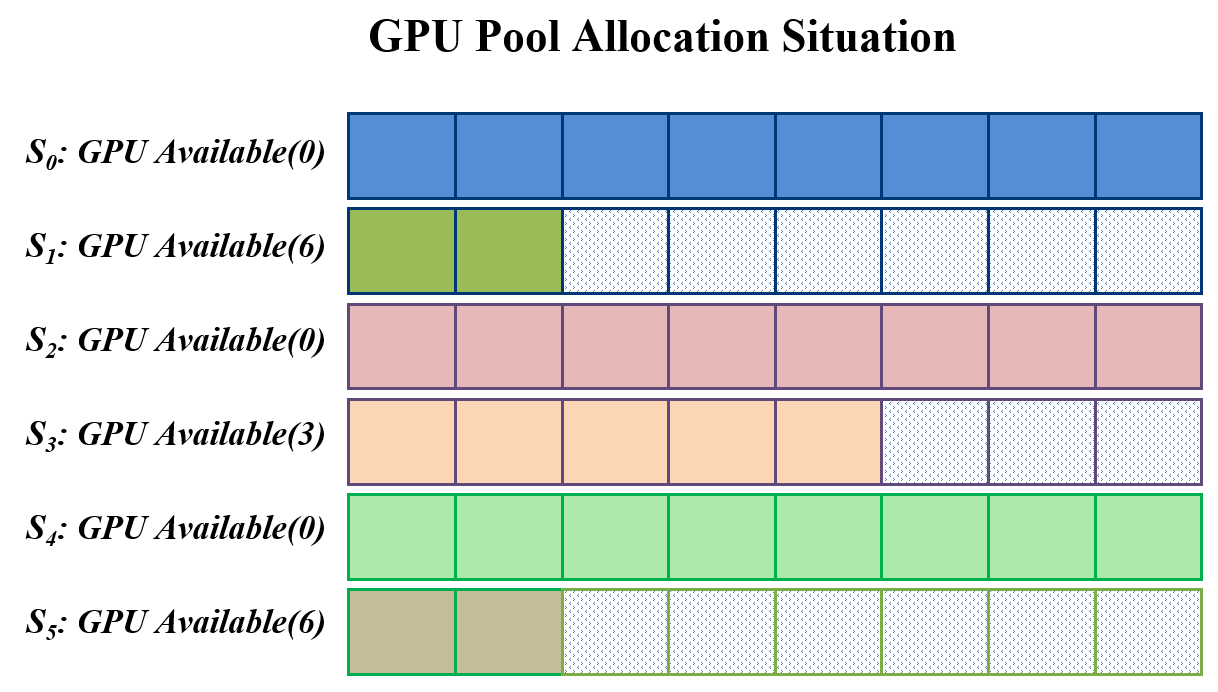
\includegraphics[width=\linewidth]{Pic/Fig_01.png}\caption{Server pool before scheduling (fragmented)}\label{fig:concept-a}\end{subfigure}

\medskip
\begin{subfigure}{0.8\columnwidth}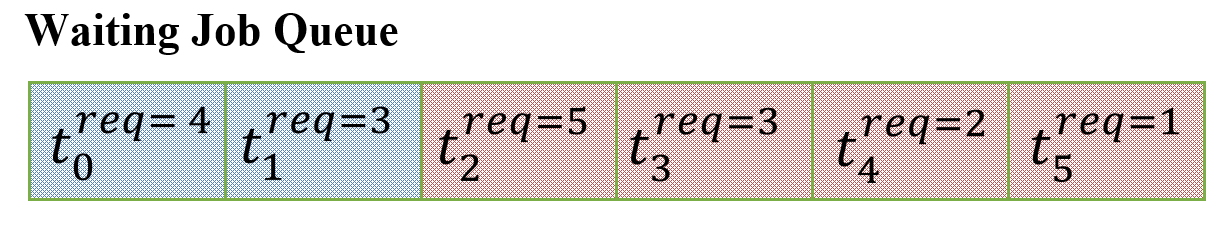
\includegraphics[width=\linewidth]{Pic/Fig_02.png}\caption{Wait queue at the same instant}\label{fig:concept-b}\end{subfigure}

\medskip
\begin{subfigure}{0.8\columnwidth}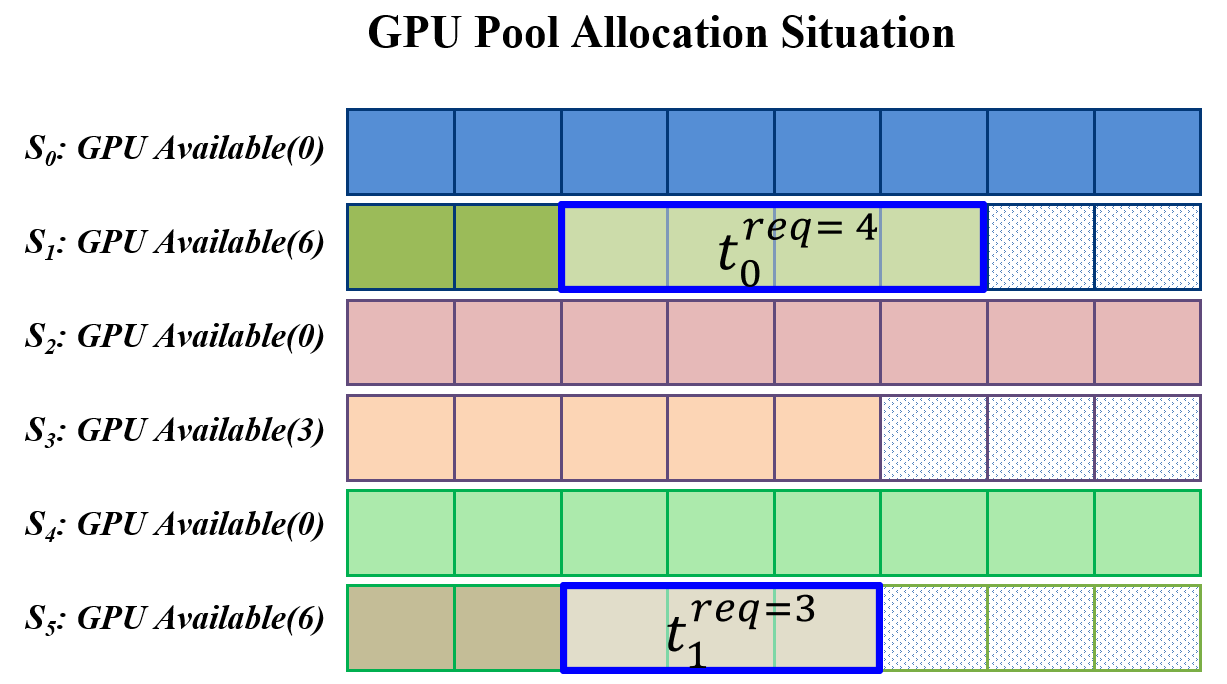
\includegraphics[width=\linewidth]{Pic/Fig_03.png}\caption{After scheduling, with $t_2$ blocked at the head}\label{fig:concept-c}\end{subfigure}

\medskip
\begin{subfigure}{0.8\columnwidth}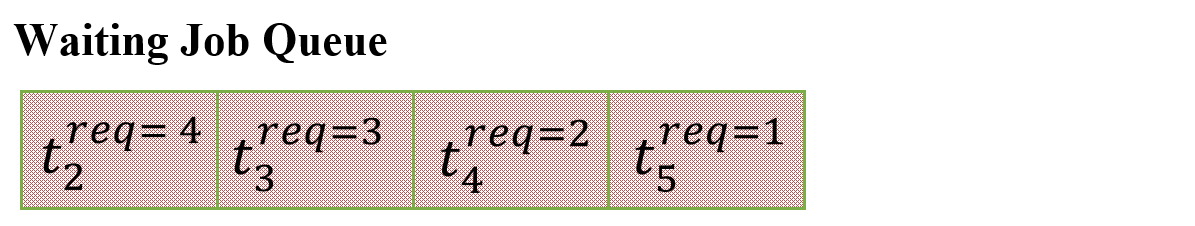
\includegraphics[width=\linewidth]{Pic/Fig_04.png}\caption{Remaining wait queue ($t_2$ through $t_5$ backlog)}\label{fig:concept-d}\end{subfigure}
\caption{Fragmentation and HOL blocking}
\label{fig:concept}
\end{figure}

Figures~\ref{fig:concept}(a) and (b) show the states of the GPU server pool and the job wait queue, respectively. In this state, a most-allocated scheduler can allocate jobs $\textit{t}_{0}$ and $\textit{t}_{1}$. Job $\textit{t}_{2}$, however, cannot be placed until other jobs complete and release GPU slots, as shown in Fig.~\ref{fig:concept}(c). Because the queue is served in strict arrival order, which is the blocking FIFO of Section~\ref{Related}, the subsequent jobs $\textit{t}_{3}$, $\textit{t}_{4}$, and $\textit{t}_{5}$ can be scheduled only after $\textit{t}_{2}$ has been scheduled.

The problem is that the pool already contains enough free GPU slots to satisfy the combined demand of $\textit{t}_{2}$ and $\textit{t}_{3}$. This is precisely HOL blocking, caused by fragmentation of the GPU server pool by previously allocated jobs. Such fragmentation forms and dissipates continuously during operation, and the worst case occurs when every GPU server has 7 free GPUs while the HOL-blocked job requests 8.

HOL blocking in GPU gang scheduling arises because allocation is both spatial and indivisible (all-or-nothing). An 8-GPU job can run only when 8 GPUs are secured simultaneously on a single server. If free GPUs are scattered across several servers, with 7 available on each, the job cannot be placed even though the aggregate capacity is sufficient. Moreover, non-preemption is the de facto standard for GPU jobs, since training jobs incur high checkpoint-and-reload costs and reshaping the resource pool is either impossible or prohibitively expensive. Starvation is therefore relieved only when a contiguous slot large enough for the job becomes available. The scheduler cannot make that slot open any sooner. What it can do is keep the large job near the head of the queue, so that when the slot finally opens, the job is in position to take it.

HOL blocking carries an efficiency cost. While the head is blocked, GPUs that the jobs behind it could use sit idle. Blocking FIFO therefore holds lower utilization than any policy that dispatches past the blocked head. On a hyper-cluster of hundreds to thousands of GPUs, even a few points of utilization are tens of GPUs idle at all times. The comparison also shows that, on the efficiency axis, dispatching past the head works. The idle GPUs are recovered almost entirely. What the comparison hides is who pays for the recovery. The job the scheduler keeps passing over falls further and further behind, and if it is large it may never run. Under every such policy, the jobs served worst are overtaken by every job that arrives after them. The efficiency cost of HOL blocking therefore has a known cure, but the cure starves large jobs, and tolerating the blocking to protect them wastes GPUs instead. It is this trade-off, rather than the blocking alone, that remains unsolved. This work aims to show that the trade-off is not binding, by removing the waste without paying the starvation.

This trade-off is not a new discovery, and neither is the standard response to it. Space-shared parallel job scheduling has assumed indivisible, non-preemptive jobs on a fragmenting pool since the JSSPP lineage\cite{feitelson1996toward}, and the answer to starvation in that setting has always been aging. Maui's XFactor and wait-time weights\cite{jackson2001maui} and Slurm's age factor raise a waiting job's priority over time, and Tetris\cite{grandl2014multi} goes furthest by folding a multi-dimensional resource-alignment score into the same decision. Yet none of these removes the trade-off. Each exposes it as a weight knob that an operator must set, and the right setting shifts with the workload. Aging as practiced also ignores whether the aged job can fit the currently free slots, so a promotion can be wasted on a job the pool cannot yet hold. The classical line thus relocates the trade-off into a tuning parameter rather than resolving it.

Prediction does not resolve it either. Arrival and completion times are unknown at scheduling time, and the non-clairvoyant setting carries competitive-ratio lower bounds of its own\cite{motwani1994nonclairvoyant}, so approaches that forestall HOL blocking by estimating the future buy that foresight with estimation error and profiling cost.

What remains open is therefore a mechanism that acts after HOL blocking occurs, reads only what the scheduling instant provides, namely queue position, resource demand, relative age, and current server occupancy, and sets its own aging weight from queue statistics instead of an operator's knob. Section~\ref{algo:intro} constructs such a mechanism, and Section~\ref{eval:robust:placement} tests whether its gains survive across Placement policies.

\section{RESOLVING HEAD-OF-LINE BLOCKING IN THE JOB QUEUE}\label{algo:intro}
A gang, in this paper, is a fixed GPU request that must be met in full and at once, what the Feitelson and Rudolph taxonomy\cite{feitelson1996toward} calls a rigid job. The word does not refer to Ousterhout's gang scheduling\cite{ousterhout1982gang}, which coordinates time slicing rather than allocation.

\subsection{SAFA Queue Reordering}
A job that later arrivals keep overtaking never reaches its turn. The median queue wait does not show this, because it reflects the many jobs that fit rather than the few that do not. A policy can report a low median and still never run those jobs. Order fairness is therefore not a nice-to-have but a production requirement: no job may be excluded indefinitely.

The goal of queue reordering is not throughput. It is to cut the queueing delay that HOL blocking imposes on the jobs behind the head while giving up as little arrival order as that cut allows. What it prevents is a queue stalled indefinitely behind one job while the backlog grows, not the completion of any particular large job, which still depends on a slot opening. Promoting jobs without restraint would simply relocate the unfairness rather than remove it, so a single weight controls how far a job's accumulated age may override its arrival order.

SAFA reorders the wait queue with the procedure in Algorithm~\ref{alg:reorder}, which runs at every scheduling pass and has three blocks. The first sweeps the server pool and updates resource fitness $R$ for each request size. The second rebases the relative ages of pending jobs and computes each adjusted priority $P^*$. The third moves the job with the largest $P^*$ to the queue head.

Resource fitness $R_j$ summarizes how well a $j$-GPU request fits the pool at the current instant. For each server $S_i$ with idle count $f_{S_i}$, a request of size $j\in\{1,\dots,M_i\}$ that fits ($j\le f_{S_i}$) scores $R_j=1$. A request that does not fit loses $0.1$ per GPU of shortfall, and the best score across all servers is retained. $R_j$ therefore ranges over $[0,1]$, and it is the one input SAFA draws from outside the queue.

The second block computes priorities. The age $A_j$ is a non-negative integer incremented by 1 whenever a new job is submitted, so it counts arrivals rather than elapsed time. Subtracting the minimum age in the queue gives the relative age $\tilde A_j=A_j-\min_k A_k$, from which each pending job's $P^*$ follows.

\begin{equation}
P^*_j = P_j + \alpha\, \tilde A_j \cdot R_j
\label{eq:01}
\vspace{2pt}
\end{equation}

The first term $P_j=1/\text{base}^{\,pos_j}$ is the arrival priority. With $\text{base}=2$, positions $pos_j=0,1,2$ yield $1$, $0.5$, and $0.25$, and larger values rank higher. The second term $\alpha\,\tilde A_j R_j$ is the priority adjustment, which multiplies how long a job has waited by how well it fits the vacant slots. The coefficient $\alpha$ sets how quickly that product can override arrival order. To put a number on that, suppose arrivals are steady enough that one age unit corresponds to ten minutes, and consider the second job in the queue, which starts at $P_j=0.5$. For it to gain $0.5$ within six hours at $R_j=1$, we need $\alpha\ge0.013889$, since $0.013889\times36\times1=0.5$.

This example, however, is a simplification that ignores the head's own adjustment. In reality the head also carries $\alpha\,\tilde A_0 R_0$, so a true inversion occurs only when the difference in the two jobs' $\tilde A\cdot R$ products exceeds the difference in their arrival priorities, that is, only when slot fitness $R$ differs between them.

The third block finds the position $i_{\max}$ of the largest $P^*$ and, unless that job already sits at the head, moves it to the front while leaving every other job in its existing relative position. Each pass moves only the single job with the highest adjusted priority to the front of the queue, because placing that job changes the pool's free slots and thereby invalidates $R$, and with it every other job's $P^*$. That job is the one that has starved the most and best fits the currently vacant GPU slots, and the positions of the remaining jobs are largely preserved.

$pos_j$ and $\tilde A_j$ are read straight from the queue, and $R_j$ combines the job's accelerator request with the free-slot count on each server into a single fitness value. All are read at the scheduling instant and none is estimated. The linear form resembles Kleinrock's time-dependent priority\cite{kleinrock1976queueing}, but only in shape. Kleinrock's conservation law assumes preemption, a single server, and steady state, none of which holds in a non-preemptive, space-shared, oversaturated gang setting. What SAFA adds to that classical form is indivisible-gang resource fitness $R$ and a coefficient normalized by queue statistics.

\begin{algorithm}
\caption{SAFA queue reordering}\label{alg:reorder}
\textbf{Input:} \\
\hspace*{4mm} Servers $S_i$ ($i{<}n$): accelerator count $M_i$, idle count $f_{S_i}$ \\
\hspace*{4mm} Pending jobs $t_i$ ($i{<}l_{wq}$): accelerator request $a_{t_i}$, age $A_i$ \\
\hspace*{4mm} Resource fitness $R_j$ ($j\in\{1,\ldots,8\}$, initially 0)
\begin{flushleft}
\textbf{Procedure:} Updated wait queue
\end{flushleft}
\begin{algorithmic}[1]
\STATE $R \gets 0$
\STATE {}
\FOR{ $i \gets 0$ to $n-1$}
    \FOR{$j \gets 1$ to $M_i$}
        \IF{$j > f_{S_i}$}
            \STATE $R_j \gets \max\{R_j,\ 1 - ( j - f_{S_i} ) \times 0.1\}$ \COMMENT{request $j$ exceeds availability $f_{S_i}$, decrease 0.1 per shortfall}
        \ELSE
            \STATE $R_j \gets 1$ \COMMENT{sufficient availability, perfect fit}
        \ENDIF
    \ENDFOR
\ENDFOR
\STATE {}
\STATE $\tilde A_i \gets A_i - \min_k A_k,\ \forall i$ \COMMENT{rebase relative ages}
\FOR{ $i \gets 0$ to $l_{wq}-1$}
    \STATE $P_i \gets 1/\text{base}^{\,i}$ \COMMENT{$\text{base}=2$}
    \STATE $P_i^* \gets P_i + \alpha\, \tilde A_i \cdot R_{a_{t_i}}$
\ENDFOR
\STATE {}
\STATE $(P_{i_{\max}}^*, i_{\max}) \gets \max(P^*)$
\IF{$i_{\max} \neq 0$}
    \STATE $WQ \gets [\,t_{i_{\max}}\,] \,\Vert\, WQ[0{:}i_{\max}) \,\Vert\, WQ[i_{\max}{+}1{:}l_{wq})$ \COMMENT{$\Vert$: concatenation; slices are half-open}
\ENDIF
\end{algorithmic}
\end{algorithm}

SAFA runs immediately before Placement and reads nothing beyond the wait queue and the current allocation state of the server pool. It is therefore a pre-placement reordering layer that leaves the core scheduler untouched, except where that scheduler performs its own queue scheduling or depends on cumulative metrics or contextual information. Because $P^*$ is computed once per job, the pass costs $O(l_{wq})$, and computing $R$ is linear in the number of servers.

\subsection{Setting the Coefficient $\alpha$ without Tuning}\label{sec:coeff}
This section defines the trade-off that $\alpha$ controls, shows that its optimum shifts far enough across workloads that no fixed value serves them all, and derives the tuning-free coefficient $\alpha_{\text{eff}}$ that reads its value from queue statistics.

\subsubsection{Trade-off Analysis and Metric Definitions}
A large $\alpha$ lets blocked jobs overtake aggressively enough to create fresh unfairness, so choosing a value means quantifying what is traded. We group cumulative waiting times by requested accelerator count and define the resulting change as accumulated distance (AD). Let $C_k$ be the class of jobs requesting $k$ accelerators, $WT_k=\sum_{j\in C_k} w_j$ the sum of waiting times before reordering, and $WT'_k$ the sum afterward. The weight $1/2^{8-k}$ gives more importance to classes with larger requests.
\begin{equation}
AD = \sum_{k=1}^8 \frac{(WT'_k - WT_k)}{2^{8-k}}
\label{eq:07}
\end{equation}

Applying the same weights to the change in the worst wait per class yields the accumulated maximum distance (AMD).

\begin{equation}
AMD = \sum_{k=1}^8 \frac{\max\limits_{j\in C_k} w'_j \;-\; \max\limits_{j\in C_k} w_j}{2^{8-k}}
\label{eq:08}
\vspace{2pt}
\end{equation}

Here $w_j$ and $w'_j$ denote waiting times before and after reordering. AD captures the overall skew in waiting times and AMD captures the worst wait within each class, so minimizing both at once targets average fairness and starvation suppression together. Both quantities, along with their min to max normalized sum in Eq.~\eqref{eq:09}, serve to build objective functions for the $\alpha$ search rather than to evaluate results. That the optimal $\alpha$ moves when the weighting or normalization changes is itself further evidence against fixed coefficients.

We search $\alpha$ over 0.01 to 1.99 in steps of 0.01 and take the value minimizing the sum of three min to max normalized metrics, namely makespan, AD, and AMD. The makespan is the time at which the last job in the trace completes. 

\begin{equation}
Obj_i^{sfa} = makespan_i^{norm} + AD_i^{norm} + AMD_i^{norm}
\label{eq:09}
\vspace{2pt}
\end{equation}

\subsubsection{Limitations of Fixed Coefficients}\label{coeff:limit}
A fixed $\alpha$ is limited because its optimum depends on the workload. We synthesize 1,000 jobs from each of eight distributions, namely normal, exponential, log-normal, gamma, beta, Weibull, uniform, and Poisson, and find the per-distribution optimum that minimizes Eq.~\eqref{eq:09} (Table~\ref{fig:motivation}). The optimum ranges from 0.22 for gamma and Poisson to 1.63 for log-normal. No single value serves every workload, so any fixed $\alpha$ is a compromise fitted to one of them, and a change in workload sends the grid search back to the start.

\begin{table}[htb!]
\centering
\caption{Optimal $\alpha$ by distribution}
\label{fig:motivation}
\footnotesize
\setlength{\tabcolsep}{4pt}
\resizebox{\columnwidth}{!}{%
\begin{tabular}{@{}l*{8}{c}@{}}
\toprule
Distribution & Normal & Exp. & Log-normal & Gamma & Beta & Weibull & Uniform & Poisson \\
\midrule
Optimal $\alpha$ & 0.53 & 0.44 & 1.63 & 0.22 & 0.26 & 0.55 & 0.50 & 0.22 \\
\bottomrule
\end{tabular}}
\end{table}

\subsubsection{Deriving the Tuning-Free Coefficient} \label{alphaeff}
The coefficient $\alpha$ in Eq.~\eqref{eq:01} sets how readily a job can overtake on the strength of its priority adjustment. Priorities run from 1 at the head down toward 0, so overtaking the head means making up a difference of at most 1. An adjustment much smaller than 1 never lets a job overtake, and one much larger lets any job overtake. A fixed $\alpha$ cannot hold that balance, because $\tilde A_j$ grows as a queue backs up while $R_j$ depends on what the pool looks like at that instant.

We take both scales from the queue itself. The mean relative age $A_{\text{ref}} = \max(1,\text{mean}(\tilde A))$, with $\tilde A_j = A_j - \min_k A_k$, is the age at which a job is ordinary for the present queue. Because the minimum is subtracted, a queue whose jobs all carry the same age has $\tilde A_j=0$ throughout and a mean of zero, and the lower limit of 1 stops that mean from driving the coefficient up without bound whenever the ages lie close together. The fitness $R_{\min}=\min_k R_k$ belongs to the request that fits worst, and it falls as the pool grows congested.

We set the coefficient to the reciprocal of the two scales.

\begin{equation}
\alpha_{\text{eff}} = \frac{1}{A_{\text{ref}}\,R_{\min}}
\label{eq:auto-alpha}
\end{equation}

Substituted into the adjustment, the coefficient separates it into two ratios.

\begin{equation}
\alpha_{\text{eff}}\,\tilde A_j\, R_j \;=\; \underbrace{\frac{\tilde A_j}{A_{\text{ref}}}}_{\text{waited vs.\ average}} \;\times\; \underbrace{\frac{R_j}{R_{\min}}}_{\text{fit vs.\ congestion}}
\label{eq:alphaeff-define}
\end{equation}

The first ratio asks how much longer than average this job has waited. The second asks how much better its request fits than the one that fits worst, a gap that widens as the pool congests. A job is promoted when both are large, so age alone does not lift a job out of starvation. A job of ordinary age whose request fits worst scores exactly 1 on both, which is the priority of the head, and every other job sits relative to that point. The adjustment therefore lands in the same range as the priorities however deep the queue is and however long its jobs have waited, and this is what leaves nothing to tune.

Raising priority with age is not new. Operating-system priority aging, vruntime equalization in Linux CFS, Tiresias\cite{gu2019tiresias}, and Slurm's multifactor age factor all do it. What differs here is how the weight is set. First, the adjustment is coupled to gang resource fitness $R_j$, which keeps the HOL culprit's priority low without a special case. Second, relative age cancels the time unit, so changing the measurement unit or period requires no conversion. Third, $\alpha_{\text{eff}}=1/(A_{\text{ref}}R_{\min})$ comes straight from queue statistics with no external constant.

\section{EXPERIMENTAL EVALUATION}\label{sec:eval}

\subsection{Scale Validation via Discrete-Event Simulation}\label{eval:sim}
We built a Python discrete-event simulator and replayed the entire Philly trace\cite{jeon2019philly}, about 111k jobs with a maximum request of 8 GPUs, which is the node boundary, on clusters of 256, 512, and 1024 GPUs. The simulation carries the per-job overheads in Table~\ref{tab:overhead}, measured on a single-node B200$\times$8 Kubernetes cluster. We implemented every policy ourselves, namely the FIFO baseline, the six Order policies (SJF, LAS, Kueue, EASY, Themis, Lucid), and the Placement policies FGD and KAI that compose with SAFA. For Tiresias, Kueue, FGD, KAI, and Lucid, whose authors released code, we cross-checked our implementations against the originals.

\begin{table}[htb!]
\centering
\caption{Per-job lifecycle overhead}
\label{tab:overhead}
\small
\resizebox{\columnwidth}{!}{%
\begin{tabular}{@{}lcccc@{}}
\toprule
\textbf{Stage} & Scheduling & Startup (solo/congested) & Teardown & \textbf{Total} \\
\midrule
\textbf{Overhead (s)} & 0.5 & 1.5 / 3.5 & 2.5 & \textbf{4.5 to 6.5} \\
\bottomrule
\end{tabular}}
\end{table}

\noindent We report seven metrics. Fairness is the bottom-1\% order-fairness score, where 100 is perfect order preservation and 0 is full inversion. Overtaken is the fraction of jobs overtaken by a majority of later arrivals. MedianWait and MaxWait are the median and maximum queue wait in seconds, with K$=10^3$ and M$=10^6$. Utilization is the average GPU allocation rate. Gini measures inequality of the wait-time distribution, with 0 meaning every job waits equally. TailRatio is the 99th percentile wait divided by the median.

Order fairness is defined per job. Let $o_k$ be the number of jobs that arrived after job $k$ but started before it, and let $\ell_k$ be the total number of jobs that arrived after $k$.
\begin{equation}
F_k = 100\cdot\Bigl(1 - \frac{o_k}{\ell_k}\Bigr)
\label{eq:order-fair}
\end{equation}
$F_k=100$ means order was preserved and $F_k=0$ means it was fully inverted. When $\ell_k=0$ we set $F_k=100$. The reported Fairness is the 1st percentile of $F_k$, that is, the score of the 1\% of jobs most severely overtaken, so higher is better. This definition follows Sabin and Sadayappan\cite{sabin2005unfairness}, who treat violations of arrival order as unfairness.

The Gini coefficient is taken over the $n$ jobs of a run. Let $u_1\le\cdots\le u_n$ be their waiting times in ascending order, so that $u_i$ is the $i$-th shortest wait and its rank $i$ serves as its weight.
\begin{equation}
G = \frac{2\sum_{i=1}^{n} i\,u_i}{n\sum_{i=1}^{n} u_i} - \frac{n+1}{n}
\label{eq:gini}
\end{equation}
$G=0$ means every job waits the same, and as $G$ approaches 1 the waiting concentrates on fewer jobs.

\subsection{Baseline Implementation and Fidelity}\label{eval:impl}
The comparators fall into three groups. Blocking FIFO is the reference against which every improvement is measured. The six Order policies (SJF, Themis, LAS, EASY, Kueue, Lucid) decide which job is served first and are direct alternatives to SAFA. The Placement axis (most-allocated, compact, round-robin, MCTS, FGD, and KAI in its binpack and spread modes) decides where a selected job runs and serves to test composability. Each implementation was checked line by line against author-released code.
\begin{itemize}
\item FIFO (blocking): dispatches jobs in strict arrival order, so a head job that cannot obtain a slot halts the jobs behind it. This is the blocking form defined in Section~\ref{Related}.
\item SJF: gives priority to jobs with shorter runtimes, taken as oracle durations from the trace.
\item LAS (Tiresias): gives priority to the job with the least accumulated GPU occupancy time. In a non-preemptive engine the attained service of pending jobs stays at 0, so the ordering key carries no information and the policy reduces to non-blocking FIFO. LAS here represents Tiresias in that degenerate form.
\item EASY: adds head-reservation backfilling to FIFO using oracle durations. We use the conservative variant, which advances only jobs finishing before time $T$. The full variant raises Fairness in one configuration but leaves the overload pattern unchanged.
\item Themis: gives priority to the job with the largest, and thus most disadvantaged, finish-time-fairness metric $r$. No public code is available, so we sort on $r$ without the round solver and inject the runtime information with 20\% random error. The approximation cannot rescue large jobs and may therefore be biased toward starvation.
\item Kueue: prioritizes VC quotas while borrowing spare resources through cohort borrowing, and is non-blocking. Its low Fairness here is the cost of that throughput-first configuration rather than a defect, and Fairness improves under StrictFIFO.
\item FGD: selects the node that produces the smallest fragmentation increase $\Delta F$ while the queue stays FCFS. We specialize it to whole-GPU gangs to isolate the effect of fragmentation-aware Placement.
\item KAI: ranks nodes by their unallocated GPU count, ascending under binpack so that jobs consolidate and empty nodes stay free for large gangs, and descending under spread. The published node score is monotone in that count, so ranking on the count alone reproduces the original selection. KAI also pipelines resources for a gang that does not yet fit, which our engine approximates with blocking admission. The reservation-respecting backfill this omits would raise KAI's throughput, not its order fairness. KAI applies no GPU-type preference, so unlike most-allocated it does not favour faster accelerators.
\item Lucid: performs non-preemptive collocation by sorting jobs with GPU-weighted SJF and packing them by sharing score. The authors' profiler is unavailable for this trace, so our implementation substitutes synthetic utilization, oracle durations, and a fixed slowdown coefficient.
\end{itemize}

\subsection{Main Results: the Efficiency and Fairness Landscape}\label{eval:main}
We evaluate the FIFO baseline, the six Order policies, and SAFA under three cluster configurations, namely 256, 512, and 1024 GPUs. Table~\ref{tab:sim-single} and Fig.~\ref{fig:cliff} present the results. The table reports SAFA twice. The SAFA (fixed $\alpha$) row holds one coefficient, $\alpha=0.13889$, across all three configurations, so it shows what a single value fitted once and left alone achieves as the cluster changes. The SAFA row uses the tuning-free coefficient $\alpha_{\text{eff}}$, recomputed from queue statistics at every pass.

\begin{table*}[htb!]
\centering
\caption{Main results: order fairness (Fairness and Overtaken), queueing delay, resource utilization, and distributional fairness (Gini and TailRatio)}
\scriptsize
\setlength{\tabcolsep}{2.5pt}
\resizebox{\textwidth}{!}{%
\begin{tabular}{@{}l rrr rrr rrr rrr rrr rrr rrr@{}}
\toprule
 & \multicolumn{3}{c}{\textbf{Fairness}} & \multicolumn{3}{c}{\textbf{Overtaken (\%)}}& \multicolumn{3}{c}{\textbf{MedianWait (s)}} & \multicolumn{3}{c}{\textbf{MaxWait (s)}} & \multicolumn{3}{c}{\textbf{Utilization (\%)}} & \multicolumn{3}{c}{\textbf{Gini}} & \multicolumn{3}{c}{\textbf{TailRatio}}  \\
\cmidrule(lr){2-4}\cmidrule(lr){5-7}\cmidrule(lr){8-10}\cmidrule(lr){11-13}\cmidrule(lr){14-16}\cmidrule(lr){17-19}\cmidrule(lr){20-22}
\textbf{Policy} & 256 & 512 & 1024 & 256 & 512 & 1024 & 256 & 512 & 1024 & 256 & 512 & 1024 & 256 & 512 & 1024 & 256 & 512 & 1024 & 256 & 512 & 1024 \\
\midrule
FIFO & 100 & 100 & 100 & 0.0 & 0.0 & 0.0 & 5.8M & 1.6M & 2 & 13.0M & 3.0M & 99K & 92 & 92 & 77 & 0.36 & 0.35 & 0.81 & 2.2 & 1.9 & 43,596 \\
SJF & 0 & 31 & 99 & 5.8 & 1.0 & 0.0 & 880 & 27 & 2 & 12.3M & 5.6M & 211K & 97 & 94 & 76 & 0.95 & 0.98 & 0.95 & 13,336 & 99,216 & 5,164 \\
LAS & 0 & 5 & 100 & 8.1 & 3.8 & 0.0 & 1.5M & 130K & 2 & 11.0M & 3.1M & 128K & 99 & 98 & 76 & 0.45 & 0.71 & 0.92 & 7.4 & 22.7 & 11,942 \\
Kueue & 0 & 0 & 100 & 7.2 & 3.8 & 0.0 & 19K & 2.1K & 2 & 12.2M & 4.9M & 224K & 98 & 95 & 77 & 0.92 & 0.94 & 0.94 & 605.3 & 1,909 & 7,971 \\
EASY & 0 & 0 & 100 & 4.4 & 3.4 & 0.0 & 5.0M & 1.3M & 2 & 12.3M & 2.8M & 86K & 92 & 93 & 77 & 0.40 & 0.41 & 0.85 & 2.4 & 2.0 & 37,687 \\
Themis & 0 & 8 & 99 & 6.4 & 1.7 & 0.0 & 3.5K & 378 & 2 & 12.0M & 4.4M & 162K & 97 & 94 & 76 & 0.94 & 0.97 & 0.94 & 3,082 & 7,665 & 5,438 \\
Lucid & 0 & 97 & 100 & 3.4 & 0.0 & 0.0 & 2.2K & 0 & 0 & 8.3M & 818K & 2 & 99 & 85 & 48 & 0.94 & 0.93 & 0.75 & 2,179 & 0.0 & 0.0 \\
SAFA (fixed $\alpha{=}0.13889$) & 88.8 & 79.0 & 99.9 & 0.0 & 0.0 & 0.0 & 4.4M & 1.2M & 2 & 11.2M & 2.5M & 94K & 98 & 97 & 77 & 0.39 & 0.36 & 0.82 & 2.5 & 1.9 & 36,752 \\
SAFA & 93.5 & 92.7 & 100.0 & 0.0 & 0.0 & 0.0 & 5.0M & 1.5M & 2 & 11.9M & 2.7M & 102K & 96 & 95 & 77 & 0.38 & 0.34 & 0.80 & 2.4 & 1.8 & 45,416 \\
\bottomrule
\end{tabular}}
\label{tab:sim-single}
\end{table*}

\paragraph{Fairness and utilization}
Fig.~\ref{fig:tradeoff} places every policy on the two axes at once. The existing policies split along a trade-off. FIFO holds Fairness at 100 but gives up GPU utilization to HOL blocking, while the others raise utilization by starving large jobs. SAFA occupies neither corner. Across the three configurations, all six Order policies fall to a Fairness of 0 under the heaviest load, whereas SAFA holds 92.7 to 93.5 (Fig.~\ref{fig:cliff}). Overtaken is 0.0\% for SAFA and for FIFO, against 3.4 to 8.1\% for the six Order policies (Table~\ref{tab:sim-single}). FIFO gives up about 7 percentage points of utilization to indivisible gangs, running at 92\% where unreserved backfilling reaches 97 to 99\%. EASY is the exception at 92\%, since its head reservation leaves it little room to backfill. SAFA recovers most of the gap at 95 to 96\% without losing order.

\begin{figure}[htb!]
\centerline{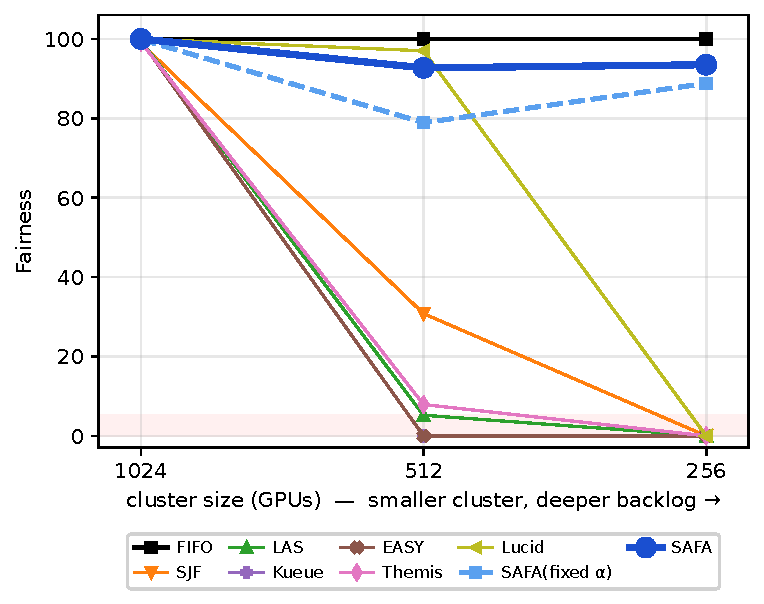
\includegraphics[width=\columnwidth]{Pic/Fig_cliff.pdf}}
\caption{Load and fairness cliff.}
\label{fig:cliff}
\end{figure}

\paragraph{Distributional fairness}
Fairness reads the tail of the order violations, so we also check the whole wait-time distribution in the 256-GPU configuration. SAFA's Gini of 0.38 sits close to FIFO's 0.36 and far below most Order baselines at 0.92 to 0.95. Its TailRatio of 2.4 contrasts with SJF at 13,336, Themis at 3,082, and Lucid at 2,179. LAS and EASY are the informative cases. Their Gini coefficients are low, 0.45 and 0.40, yet their Fairness is still 0, which means the waiting is spread evenly while arrival order is not respected. Neither dimension substitutes for the other, and SAFA's advantage does not rest on a single metric.

\begin{figure}[htb!]
\centerline{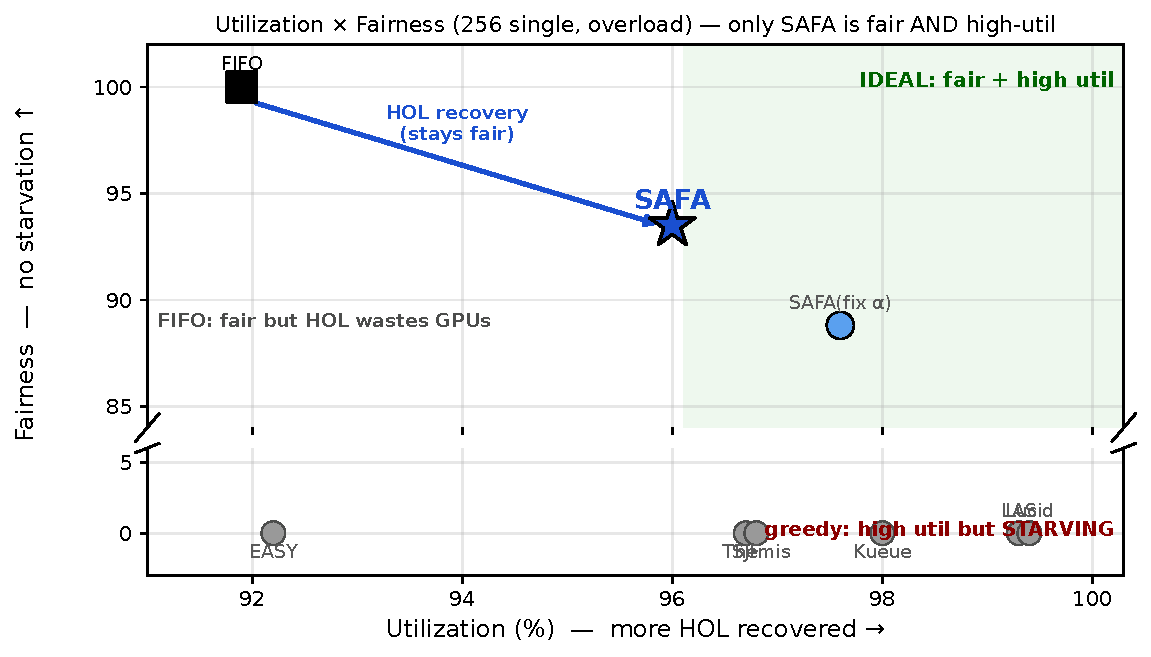
\includegraphics[width=\columnwidth]{Pic/Fig_tradeoff.pdf}}
\caption{Utilization and fairness trade-off.}
\label{fig:tradeoff}
\end{figure}

\begin{table}[htb!]
\centering
\caption{Best fixed $\alpha$ found by grid search, refitted per configuration, versus the tuning-free coefficient}
\label{tab:ablation-grid}
\footnotesize
\begin{tabular}{@{}ll@{\hspace{0.8em}}rr@{\hspace{0.8em}}rr@{}}
\toprule
 & & \multicolumn{2}{c}{\textbf{Optimal fixed $\alpha$}} & \multicolumn{2}{c}{\textbf{SAFA}} \\
\cmidrule(lr){3-4}\cmidrule(lr){5-6}
 & \textbf{GPU} & Fairness\,($\alpha^\ast$) & MedianWait & Fairness & MedianWait \\
\midrule
 & 256  & 88.8\,(0.14) & 4.4M & \textbf{93.5} & 5.0M \\
                     & 512  & 90.6\,(0.9)  & 1.3M & \textbf{92.7} & 1.5M \\
                     & 1024 & 100.0\,(0.01) & 2    & \textbf{100.0} & 2    \\
\bottomrule
\end{tabular}
\end{table}

\paragraph{Tuning-free effect}
Table~\ref{tab:ablation-grid} compares the tuning-free coefficient against the best fixed $\alpha$ a grid search can find. At each configuration on the Philly trace we sweep $\alpha$ over sixteen points from 0.01 to 2.0 and keep the one that reaches the highest Fairness, which is the strongest result any fixed coefficient can reach there. SAFA still leads in every configuration, at 93.5 against 88.8, 92.7 against 90.6, and 100.0 against 100.0. The score gap is not the point. The best $\alpha$ itself moves from 0.14 to 0.9 to 0.01 as the cluster size changes, so a fixed coefficient has to be refitted for each configuration, while SAFA reads its coefficient from the queue and needs no such search. What refitting is worth is visible in Table~\ref{tab:sim-single}. The single $\alpha=0.13889$ used there is the best available choice at 256 GPUs, where it scores 88.8, but carrying that same value to 512 GPUs scores 79.0, against 90.6 for a coefficient refitted to that configuration. SAFA reaches 92.7 at 512 GPUs without being told anything about it. Section~\ref{eval:robust:trace} shows the same on workloads it was never fitted to.

\subsection{Generalization to Independent Traces}\label{eval:robust:trace}
The results so far come from one trace. We therefore repeat the evaluation on two further public traces that share no lineage with Philly. The first is the Venus cluster trace from the Helios\cite{hu2021helios} datacenter (SenseTime, SC'21, 125,303 jobs, one overloaded 80-GPU configuration). We use 123,969 jobs after excluding 1{,}334 that exceed the 80-GPU capacity and therefore cannot be placed by any policy. The pattern repeats. Every Order baseline falls to a Fairness of 0 with Overtaken between 6.4 and 22.8\%, while SAFA holds Fairness at 97.6 with Overtaken at 0.0, and fixed $\alpha$ reaches 92.5. The second is the Alibaba PAI\cite{weng2022mlaas} trace (NSDI'22), a seed-42 16.4\% subsample that yields 120,105 jobs, with the load multiplier matched to Philly, and it behaves the same way.

Table~\ref{tab:trace3} collects all three. Under a single overloaded configuration the Order baselines run from 3.4 to 22.8\% Overtaken, reaching double digits on Helios and Alibaba, while SAFA keeps Overtaken at 0.0 and Fairness at 93.5, 97.6, and 99.9 on Philly, Helios, and Alibaba respectively. No retuning was performed between traces.

\begin{table}[htb!]
\centering
\caption{Generalization across independent large-scale traces}
\label{tab:trace3}
\scriptsize
\setlength{\tabcolsep}{4pt}
\resizebox{\columnwidth}{!}{%
\begin{tabular}{@{}l@{\hspace{0.6em}}rr@{\hspace{0.9em}}rr@{\hspace{0.9em}}rr@{}}
\toprule
 & \multicolumn{2}{c}{\textbf{Philly}} & \multicolumn{2}{c}{\textbf{Helios}} & \multicolumn{2}{c}{\textbf{Alibaba}} \\
\cmidrule(lr){2-3}\cmidrule(lr){4-5}\cmidrule(lr){6-7}
\textbf{Policy} & Overtaken & Fairness & Overtaken & Fairness & Overtaken & Fairness \\
\midrule
FIFO          & 0.0   & 100  & 0.0  & 100  & 0.0  & 100 \\
SJF           & 5.8   & 0    & 16.1 & 0    & 6.0  & 0 \\
LAS/Kueue     & 7 to 8  & 0    & 22.8 & 0    & 10.6 & 0 \\
EASY          & 4.4   & 0    & 8.9  & 0    & 13.4 & 0 \\
Themis        & 6.4   & 0    & 15.2 & 0    & 6.6  & 0 \\
Lucid         & 3.4   & 0    & 6.4  & 0    & 5.7  & 0 \\
SAFA (fixed $\alpha{=}0.13889$) & 0.0 & 88.8 & 0.0 & 92.5 & 0.0 & 94.7 \\
\textbf{SAFA} & \textbf{0.0} & \textbf{93.5} & \textbf{0.0} & \textbf{97.6} & \textbf{0.0} & \textbf{99.9} \\
\bottomrule
\end{tabular}}
\end{table}

\subsection{Placement Composability}\label{eval:robust:placement}
Since SAFA acts before Placement, it can sit in front of any Placement policy. For each of the seven, namely most-allocated, compact, round-robin, MCTS, FGD, KAI binpack, and KAI spread, we measure the policy under FIFO and then under SAFA (Table~\ref{tab:placement}, one overloaded 256-GPU configuration, same seven metrics as the main results).

Fragmentation costs something under every placement, and the amount tracks how widely the policy scatters jobs. Under FIFO, utilization falls from 91.9\% with most-allocated to 89.3\% with KAI spread, and the median wait rises from 5.8M\,s to 6.2M\,s, because scattered free GPUs leave no node able to hold an 8-GPU gang in full.

SAFA raises utilization and shortens the wait under all seven policies. Filling vacant node slots with jobs that fit brings utilization back to 94.7 to 96.5\%, a gain of 3.7 to 5.8 percentage points, and cuts the median wait by 11 to 18\%. Order fairness is what it spends: Fairness falls from FIFO's 100 to 91.8 to 93.7, while Gini moves from 0.36 to 0.39 and TailRatio from 2.23 to 2.42. Those are small displacements next to the 0 that every Order baseline records in Table~\ref{tab:sim-single}. The recovery is largest where the placement scatters most aggressively. Under KAI spread, utilization rises from 89.3\% to 95.1\%, a gain of 5.8 percentage points (Fig.~\ref{fig:placehol}). SAFA therefore does more than tolerate the placement policy beneath it. It returns the utilization that fragmentation took, and it does so most where fragmentation is worst.

\begin{figure}[htb!]
\centerline{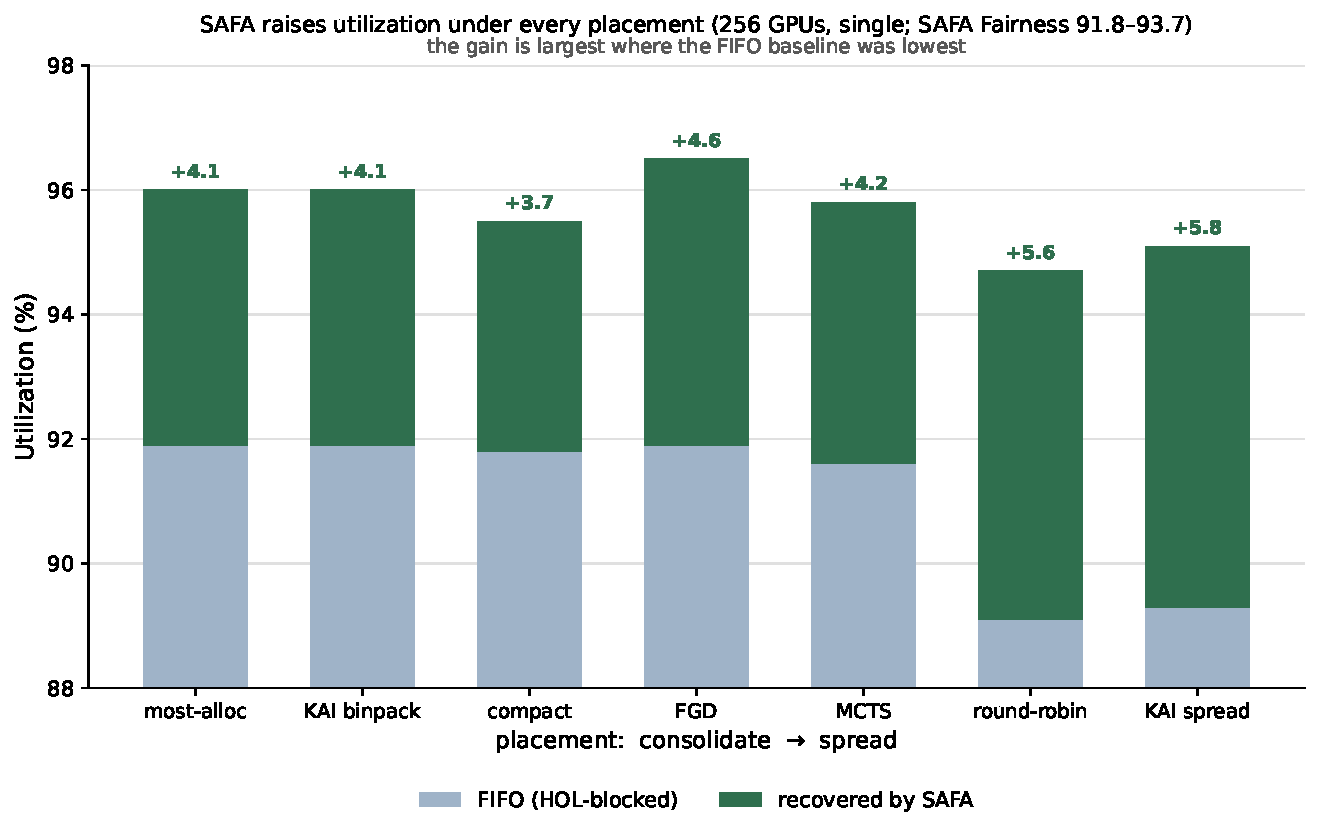
\includegraphics[width=\columnwidth]{Pic/Fig_placement_hol.pdf}}
\caption{HOL recovery under varying levels of fragmentation.}
\label{fig:placehol}
\end{figure}

\begin{table}[htb!]
\centering
\caption{Metrics before and after composing SAFA with Placement policies (single overloaded 256-GPU configuration)}
\label{tab:placement}
\resizebox{\columnwidth}{!}{%
\begin{tabular}{@{}ll rrrrrrr@{}}
\toprule
\textbf{Placement} & & \textit{MedianWait} & \textit{MaxWait} & \textit{Fairness} & Overtaken & \textbf{Utilization} & Gini & TailRatio \\
\midrule
\multirow{2}{*}{most-allocated} & FIFO & 5.8M & 13.0M & 100.0 & 0.0 & 91.9 & .36 & 2.23 \\
                                & SAFA & 5.0M & 11.9M & 93.5 & 0.0 & \textbf{96.0} & .38 & 2.36 \\
\multirow{2}{*}{compact}        & FIFO & 5.8M & 13.0M & 100.0 & 0.0 & 91.8 & .36 & 2.23 \\
                                & SAFA & 5.2M & 12.0M & 93.1 & 0.0 & \textbf{95.5} & .38 & 2.32 \\
\multirow{2}{*}{round-robin}    & FIFO & 6.1M & 13.8M & 100.0 & 0.0 & 89.1 & .36 & 2.24 \\
                                & SAFA & 5.1M & 12.4M & 91.8 & 0.0 & \textbf{94.7} & .39 & 2.42 \\
\multirow{2}{*}{MCTS}           & FIFO & 5.8M & 13.1M & 100.0 & 0.0 & 91.6 & .36 & 2.24 \\
                                & SAFA & 5.1M & 12.1M & 93.7 & 0.0 & \textbf{95.8} & .38 & 2.35 \\
\midrule
\multirow{2}{*}{FGD}            & FIFO & 5.8M & 13.1M & 100.0 & 0.0 & 91.9 & .36 & 2.24 \\
                                & SAFA & 5.0M & 12.0M & 93.5 & 0.0 & \textbf{96.5} & .38 & 2.37 \\
\multirow{2}{*}{KAI binpack}    & FIFO & 5.8M & 13.0M & 100.0 & 0.0 & 91.9 & .36 & 2.23 \\
                                & SAFA & 5.0M & 11.9M & 93.5 & 0.0 & \textbf{96.0} & .38 & 2.36 \\
\multirow{2}{*}{KAI spread}     & FIFO & 6.2M & 13.8M & 100.0 & 0.0 & 89.3 & .35 & 2.23 \\
                                & SAFA & 5.1M & 12.3M & 91.8 & 0.0 & \textbf{95.1} & .39 & 2.42 \\
\bottomrule
\end{tabular}}
\end{table}

\subsection{Real-Cluster Validation (B200)}\label{eval:b200}
The simulator models the queue but not the Kubernetes admission and binding path, so we cross-validate on a single-node NVIDIA B200$\times$8 cluster running K8s v1.31. The workload is a 500-job Philly sample replayed with the time axis compressed and nothing else changed, which preserves the bursty submission pattern of the original. At peak, pending demand reaches 12$\times$ the 8-GPU capacity and 440 of the 500 jobs wait at once, a backlog deep enough for age promotion to matter. Each job ran as a sleep stub that held real GPUs and traversed creation, gating, and binding, giving 6 runs $\times$ 500 jobs $=$ 3{,}000 real Pods across all policies and repetitions. The experiment tests the admission and binding path and excludes computation and communication.

The queue behavior carries over. Under burst overload SAFA held Fairness at 82.8 with Overtaken at 0.0\% and a deviation of $\pm$0.2 across repetitions, while a control run that kept dispatching later jobs regardless of the head's wait collapsed to 3.8. Preserving head order is what separates the two.

A single node cannot exhibit fragmentation across nodes, and resource fitness therefore varies little, so this setup exercises the ordering behavior rather than the fragmentation recovery measured in simulation.

\subsection{Limitations}\label{eval:threats}
Three limitations bound what the results above establish, and the figures should be read as trends rather than absolute values.

First, measurement and modeling scope. Real-cluster validation covers burst replay on one B200$\times$8 node for SAFA, FIFO, and the control run only. A measured comparison of all Order policies, and end-to-end measurement of multi-node fragmentation, remain future work. We did not model network or inter-job interference, and we did not examine throughput differences across job types. Extending $R$ to per-type, node-group, and multi-dimensional resource settings is a prerequisite for that work.

Second, workload and comparison scope. The main evaluation rests on Philly with Helios and Alibaba as support, and all three are finite samples. SOTA schedulers such as Sia are absent because the decision variables they need do not exist in these traces. What we claim is a pre-placement reordering layer that requires no prediction, not superiority over every scheduler.

Third, metric bias. Fairness rewards policies that preserve arrival order, which is the property SAFA is built around, so it cannot be the only evidence. We therefore cross-checked against Gini, TailRatio, and Overtaken in Table~\ref{tab:sim-single}, which measure different things, and the advantage holds under overload. The headline contrast, a Fairness near 0 for the Order baselines against 92.7 to 93.5 for SAFA, is an order-of-magnitude difference that no single metric choice produces on its own.

These conclusions do not rank the policies absolutely. They show where the fairness and utilization trade-off appears and how sharply it bites as load rises.

\FloatBarrier

\section{CONCLUSIONS AND FUTURE WORK}\label{conclu}

This paper presented SAFA, a pre-placement reordering layer that touches only the Order stage to prevent the indefinite exclusion that HOL blocking causes in GPU server pools. We evaluated it in a discrete-event simulator across three traces (Philly, Helios, and Alibaba PAI) on clusters of 256 to 1024 GPUs, against FIFO and six Order policies, composed it with seven Placement policies, and cross-validated on an NVIDIA B200$\times$8 Kubernetes cluster. Unlike recent scheduling policies that require runtime estimates, performance profiles, or solvers, SAFA reads only quantities available at the scheduling instant, namely queue position, resource demand, relative age, and current server occupancy, and it layers over a wide range of schedulers.

Under the heaviest overload, the Fairness of all six Order policies falls to 0 while SAFA holds 91.8 to 93.7 across configurations and Placement policies. It cuts the median wait by 7 to 13\% against FIFO and lifts utilization from 92\% to 95 or 96\%, so the fairness costs no throughput. The same pattern recurs on Helios and Alibaba. Under light contention the picture differs, and collocation policies such as Lucid can be both faster and fairer. It is as load rises that the Order baselines lose order fairness and size-selective policies starve large jobs, and SAFA is the only policy here that holds both dimensions without predicting anything.

The coefficient $\alpha$ is the mechanism behind that balance. A fixed value has to be searched for, and its optimum moves substantially with the workload. SAFA computes it instead from the relative ages already in the queue and the resource fitness $R$ already read from the pool, so it adapts to workload change without a new grid search.

Two directions follow. This work covers GPU gang traces only, so extending the evaluation to classical parallel-job traces in the Standard Workload Format would connect it to the HPC batch-scheduling literature. More pressing, the B200 measurements confirm that SAFA prevents burst-overload exclusion on the real admission and binding path, at a Fairness of 82.8 with Overtaken at 0.0\%, but a single node cannot reproduce multi-node fragmentation. Expanding the real-cluster measurement to several nodes is the most important next step.

\FloatBarrier
\section*{ACKNOWLEDGMENT}
The authors received no financial support from any institution for this study.

Disclosure of generative AI use. In accordance with IEEE recommendations, the authors disclose that generative AI tools were used only in an auxiliary role during preparation of this paper. Their use was limited to sentence polishing and language editing, figure generation, experiment-reproduction scripts, and assistance with organizing results. The conception of the research, the design of the algorithm, and the execution and interpretation of the experiments were carried out by the authors. The authors reviewed and revised all AI-assisted content and bear full responsibility for the content of the publication.

\bibliographystyle{IEEEtran}
\bibliography{sn-bibliography}
%% if required, the content of .bbl file can be included here once bbl is generated
%%\input sn-article.bbl

% Author biographies --- to add a photo, replace IEEEbiographynophoto with
% \begin{IEEEbiography}[{\includegraphics[width=1in,height=1.25in,clip,keepaspectratio]{photo}}]{Name}.
% Fill in the XXXX/XX placeholders with actual degrees and years.
\begin{IEEEbiography}[{
\includegraphics[width=1in,height=1.25in,clip,keepaspectratio]{Pic/bio_kyunam_cho.jpg}}]{Kyunam Cho}~is a Research Fellow at LG Uplus in Seoul and a Ph.D. candidate in computer science at Korea University in Seoul, Korea. From 2000 to 2021, he worked as a software developer and software architect at Samsung Electronics. From 2021 to 2022, he worked as a software architect at Hyundai Card Company.

His primary research areas are high-performance computing (HPC) and HPC-based software platforms. At Samsung Electronics, he built and operated thousands of GPGPU-based machine learning systems. His current interests include large language model operations, known as LLMOps, federated learning, and chaos engineering for public-cloud-based platforms. He is the author of a book on machine learning and has published papers in Computer Physics Communications.

\end{IEEEbiography}

\begin{IEEEbiography}[{
\includegraphics[width=1in,height=1.25in,clip,keepaspectratio]{Pic/bio_younghwan_jin.jpg}}]{YoungHwan Jin}~received the B.S. and M.S. degrees in computer science from Yonsei University.
His research interests include distributed systems and cloud-native architectures, with particular emphasis on resource allocation for distributed GPU inference and scalable machine learning operations in edge environments.

\end{IEEEbiography}

\begin{IEEEbiography}[{
\includegraphics[width=1in,height=1.25in,clip,keepaspectratio]{Pic/bio_heonchang_yu.jpg}}]{Heonchang Yu}~is a Professor in the Department of Computer Science and Engineering at Korea University, Seoul, Korea. He received the M.S. and Ph.D. degrees in computer science from Korea University in 1991 and 1994, respectively. He has been a Professor at Korea University since 1998 and was a Visiting Professor in the Department of Electrical and Computer Engineering at the University of Texas at San Antonio, TX, USA, from 2019 to 2020. He leads the Distributed and Cloud Computing Laboratory at Korea University.

His research interests include cloud computing, virtualization (including GPU virtualization), distributed systems, fault-tolerant systems, and edge-cloud technologies that support real-time processing. He has served as an editor of the Korean Institute of Information Scientists and Engineers since 2007.
\end{IEEEbiography}

\end{document}
